This Chapter presents the general background and fundamental concepts related to the domain problem that is addressed in this thesis. At the first section (\autoref{sec:cscl-and-scripted-collaboration}), an overview of CSCL field and scripted collaboration is presented to provide a most comprehensive and clear understanding about the research context. This section also describes in detail the motivation problem caused by the scripted collaboration when CL activities are orchestrated and structured by CSCL scripts, as well as, the related works and current computer-based solutions to deal with this problem. The \autoref{sec:gamification} elaborates an overview of gamification, and the best practices and theories related to this technology. Furthermore, the related works that use gamification in the context of CSCL and other contexts to deal with the motivation problem are presented in this section. Finally, the \autoref{sec:ontologies-and-ontology-engineering} presents the fundamentals of ontologies and ontology engineering. This sections also discusses how ontologies is currently used to support the systematic formalization of theory-based knowledge, and how this formalization, in the field of artificial intelligence in education, is used to overcome some problems that are similar to those that must be solved to provide a computational support in the gamification of CL scenarios with theoretical justifications based on the best practices and theories related to gamification. 

\section{CSCL and Scripted Collaboration}
\label{sec:cscl-and-scripted-collaboration}

Although CL has a long history in education, it is not until the early 1990s that the research field dedicated to study how to provide support for the CL through the use of Internet and computational technology had gained attention and strength \cite{StahlKoschmannSuthers2006}. Such research field known as Computer-Supported Collaborative Learning (CSCL) is a multidisciplinary field that combines studies from the cognitive psychology education and from the computer science to effectively enhance the CL process through the use of computational technology \cite{HoppeOgataSoller2007}.

The general aim of CSCL field is to develop technologies to support or create situations in which two or more students learn together through the interaction among them \cite{Dillenbourg1999}. In these situations, the learning outcomes is consequence of students' interactions and how these interactions affect the individual learning for each one of the students. In consequence, to enable a well-though-out design of CL, the CSCL scripts have been proposed by the CSCL community as the technology to facilitate the social and cognitive processes of learning by describing the way in which the learners will interact with each other in a CL scenario \cite{HarrerKobbeMalzahn2007}.

\subsection{CSCL Scripts}
\label{sec:cscl-scripts}

CSCL scripts are the technology that describes how to structure and orchestrate the CL process to attain a set of pedagogical objectives defined by an instructional design \cite{DillenbourgJermann2007}. Such description is provided in the CSCL scripts through prescribed instructions that indicates how to facilitate the social and cognitive processes in group activities \cite{Dillenbourg2002}. These prescribed instructions are defined by instructors, like teachers or instructional designers, as a way to attain a set of learning goals, and they indicate the way in which students should collaborate, they constrain the interactions among the participants, they specify the roles for the participants, they indicate the distribution of task, tools, and resources used in the CL process.

In order to narrow the number of elements used to describe the CSCL scripts, and provide a common and sharable description of CSCL scripts, \citeonline{KobbeWeinbergerDillenbourgHarrerHamalainenHakkinenFischer2007} propose a framework that is currently wide accepted by the community as the common specification to describe the CSCL scripts using natural language. This framework formalizes the CSCL scripts as a set of components and mechanisms illustrate in \autoref{fig:components-and-mechanisms-of-cscl-scripts}.


\begin{figure}[htb]
 \caption{Components and mechanisms of CSCL scripts}
 \label{fig:components-and-mechanisms-of-cscl-scripts}
 \centering
 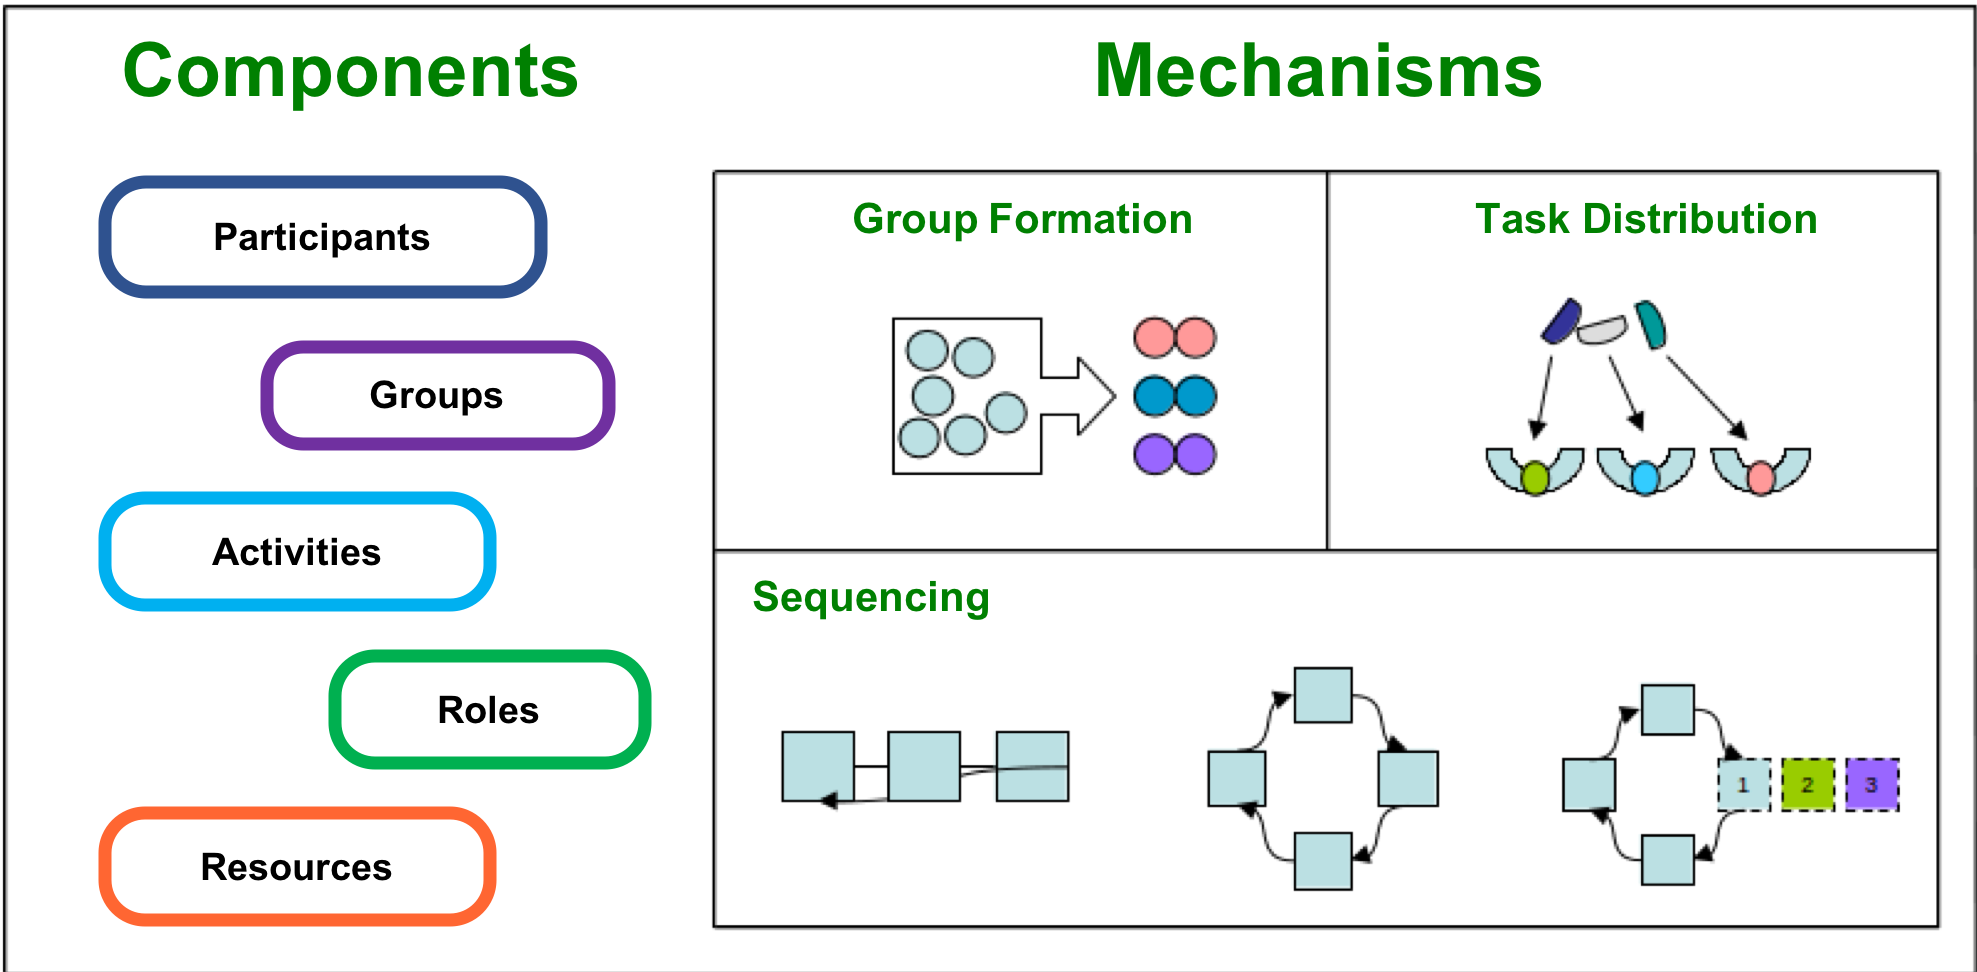
\includegraphics[width=0.95\textwidth]{images/components-and-mechanisms-of-cscl-scripts}
 \fadaptada{Fischer2007}
\end{figure}

The structural \emph{components} of CSCL scripts are the participants, groups, activities, roles and resources. The component of \emph{participants} is used to describe the participants, such as learners, monitors, and teachers. Although this description can be abstract or concrete and simple or complex, it is often presented in a simple manner with rules that indicate conditions to participate in the CL process. The component of \emph{activities} describes what will be performed by the participants in the CL process to attain the learning goals defined by the instructional designers. The component of \emph{roles} describes the privileges, obligations and expectations of participants in the CL process. The component of \emph{groups} of participants defines through hierarchical structures how the students are grouped according to the participants' characteristics. The component of \emph{resources} describes the learning objects (e.g. content, material, and tools) that can be used by the participants during the CL process.

The \emph{mechanisms} of CSCL scripts are the group formation, component distribution and sequencing. The mechanism of \emph{group formation} consists in the specifications of how the participants will be distributed over the groups. The mechanism of \emph{task distribution} provides the specification about how the components of scripts are distributed over groups using the mapping of groups, activities, roles, and resources. The mechanism of \emph{sequencing} consists in the definition of how the components and groups defined in scripts are distributed over time. In general, this sequencing describes the execution order of activities in the CL process.

\autoref{qua:social-script-framework-kobbe} shows the description of social script \cite{WeinbergerErtlFischerMandl2005} using the framework proposed by \citeonline{KobbeWeinbergerDillenbourgHarrerHamalainenHakkinenFischer2007}. In this example, the CL scenarios orchestrated by the social script foster the acquisition of knowledge through a set of case studies (\emph{resources}) that are analyzed and reviewed by the students groups. The number of students in each group is equal to the number of case studies, and the ideal number is three. In the first step of sequencing, each learner playing the \emph{analysis} role writes down an analysis of case study, and then, he critiques the analyses made by other learners playing the \emph{critics} role. In the second step of sequencing, each learner revises his/her own analysis, taking into consideration the critiques received by the other learners in the case group.

\begin{quadro}[htb]
\caption{Social script describes using the framework proposed by  \citeonline{ KobbeWeinbergerDillenbourgHarrerHamalainenHakkinenFischer2007}}
\label{qua:social-script-framework-kobbe}
\centering
\footnotesize
\begin{tabular}{l p{12cm}}
\toprule
\multicolumn{2}{l}{\textbf{Structural components:}} \\ \midrule
\textbf{Participants:} &
A number of participants that must be divisible by the number of case studies.  \\
\textbf{Groups:} &
Case groups \\
\textbf{Activities:} &
(a) Applying theoretical concepts to the case study and constructing arguments \\
 &
(b) Critiquing initially scaffolder with prompts for eliciting clarification, identifying conflicting views and constructing counter-arguments \\
\textbf{Roles:} &
\emph{Analyst} and \emph{Critic} \\
\textbf{Resources:} &
Case studies (minimal number is three case studies) \\
\toprule
\multicolumn{2}{l}{\textbf{Mechanisms}:} \\ \midrule
\textbf{Group formation:} &
All participants are grouped by the number of case studies. Each participant becomes member of all case groups although with different roles in each. Each participant is the responsible analyst for one case study and critic for all other cases \\
\textbf{Task distribution:} &
Each case group receives one case study, and the roles are distributed in a way that each participant assumes the role of analyst in one case group and the role of critic in all other case groups \\
\textbf{Sequencing:}
& - the analyst writes an analysis of case study. (a) \\
& - wait for all case group analysts to be done, and writes a critique for the analysis of case study. (b) \\
& - wait for all case group critics to be done, and the analyst considers each critique and writes a reply to each. (a) \\
& - wait for all case group analysts to be done each critic in turn reads the reply and writes a second critique. (b) \\
& - wait for all case group critics to be done... the analyst considers all critiques and revises the analysis of case study (a) \\
\bottomrule
\end{tabular}
%\fadapted{KobbeWeinbergerDillenbourgHarrerHamalainenHakkinenFischer2007}
\end{quadro}


Having the description of CSCL scripts only in natural language does not allow the computers programs to interpret them, and to run a CL scenario following the instructions indicated by the scripts without human intervention. Therefore, to represent the CSCL scripts in a computer readable manner, the IMS-Learning Design\footnote{\url{http://www.imsglobal.org/learningdesign/}} (IMS-LD) specification has been adopted by different tools, such as (web)COLLAGE \cite{Hernandez-LeoVillasclaras-FernandezAsensio-PerezDimitriadisJorrin-AbellanRuiz-RequiesRubia-Avi2006,Villasclaras-FernandezHernandez-LeoAsensio-PerezDimitriadis2013}, CIAN \cite{MolinaRedondoOrtega2012}, LeadFlow4LD \cite{Palomino-RamirezBote-LorenzoAsensio-PerezDimitriadis2008}, NUCLEO \cite{SanchoFuentes-FernandezFernandez-Manjon2008}, CoLearn \cite{StylianakisArapiMoumoutzisChristodoulakis2013}, CeLS \cite{RonenKohen-Vacs2009}, and LAMS \cite{Romero-MorenoOrtegaTroyano2007}, as the language to describe CSCL scripts.
 
Despite the benefits that brings  the use of the IMS-LD specification to represent CSCL scripts, several researchers had indicated that this language is insufficient to fully support the modeling of CSCL scripts \cite{AlharbiAthaudaChiong2014, CaeiroAnidoLlamas2003}. Of course, the purpose of IMS-LD specification is not to provide a full support for describing CSCL scripts in a computer-readable manner, the IMS-LD has been developed as a neutral, generic and flexible educational modeling language to describe a wide range of pedagogies approaches (the teaching strategies, pedagogical goals and their associated activities) \cite{Koper2005}. In this sense, to support the representation of CSCL scripts in a computer-readable manner, a wide variety of extensions on the IMS-LD elements has been proposed in by several researchers \cite{Bote-LorenzoVaquero-GonzalezVega-GorgojoDimitriadisAsensio-PerezGomez-SanchezHernandez-Leo2004, LeoPerezDimitriadis2004, MagnisalisDemetriadis2012, MiaoHoeksemaHoppeHarrer2005, Vega-GorgojoBote-LorenzoGomez-SanchezDimitriadisAsensio-Perez2005}.

Instead, to simply provide a computer-readable representation of CSCL scripts, the work of \citeonline{Isotani2009} proposes the formalization of these scripts in a computer-understandable manner through the use of ontologies. This solution consists in a set of ontological structures that makes the description of CSCL scripts more semantically-rich, allowing the explicit specification of learning goals, purposes, and other relevant information that cannot be represented using the IMS-LD specification, i.e., learning strategies, group goals, interaction patters from learning theories. Providing this formalization in the CL ontology, \citeonline{IsotaniMizoguchiIsotaniCapeliIsotanideAlbuquerqueBittencourtJaques2013} demonstrates that intelligent-theory aware systems can interpret these scripts and provide advice and recommendation to support for the modeling of learners' development \cite{InabaIkedaMizoguchi2003}, the formation of effective groups \cite{IsotaniMizoguchi2008a}, and the instructional design of CL activities \cite{IsotaniMizoguchiIsotaniCapeliIsotanideAlbuquerqueBittencourtJaques2013}.

\subsection{Levels of Abstraction and Granularity of CSCL Scripts}
\label{sec:level-of-abstraction-and-granularity-of-cscl-scripts}

CSCL scripts have different levels of abstraction and granularity in the description of CL scenarios \cite{Dillenbourg2002, DillenbourgJermann2007, Villasclaras-FernandezIsotaniHayashiMizoguchi2009}. This classification of scripts in two dimension, abstraction and granularity, gives them an enormous flexibility to be reused in the instructional design process of CL scenarios, and it also allows the use of multiple scripts to describe different aspects of CL scenario in separated scripts. Whereas the levels of abstraction classify a script according to the completeness of elements described by them (from the most abstract to the most concrete), the levels of granularity classify the scripts according to the aggregation level of elements described by them (from the most coarser grained to the finest grained).

According to \citeonline{DillenbourgJermann2007}, a CSCL script can be classified in one of the four levels of abstraction defined as follows as:

\begin{description}
\item[\emph{Script Schemata}:] are scripts use to describe the core instructional design principles whereby is expected to trigger interactions among participants in the CL process. In this sense, these scripts are defined in a content free didactic form, so that they can be used to describe patterns of CL. Examples of script schemata are the Jigsaw script \cite{Aronson1978, KordakiSiempos2010}, conflict script \cite{WeinbergerErtlFischerMandl2005}, and reciprocal script \cite{King2007}. The jigsaw script describes a CL scenario in which the principle of interaction consists in the grouping and re-grouping of participants with complementary information to share their knowledge. The conflict script describes a CL scenario to group learners with contradictory knowledges or opinions to instigate the discussion. The reciprocal script describes a CL scenario that assigns alternate roles to the students for facilitating questioning and tutoring activities.

\item[\emph{Script Classes}:] are specialization of scripts schemata for a specific learning context. This specialization is not absolute complete, so that script classes are independent in the content-domain and student data. The script classes cover a range of scripts that describe variations of a prototype with particular details related to a specific learning context of a script schemata to facilitate its adoption. These details are, for example, the number of participants, and the king of content (matter) that will be taught. In this sense, a script class is based in a script schemata to describe CL scenarios for a specific learning context. For instance, the Universanté Script \cite{DillenbourgJermann2007} is a script class based on Jigsaw schema that was designed to describe CL scenarios for learning contexts with different thematic groups and participants from different nations.

\item[\emph{Script Instances}:] are scripts in which the content-domain are specified for a particular situation. A script instance is more concrete than a script class, and it has been instantiated from a script schema or class to be reusable more or less by teachers who only need to define participants' data. These scripts are more concrete that script classes, but they are independent in the particularities of students and learning environment.

\item[\emph{Script Sessions}:] are scripts in which the content-domain and participants data are specified to be directly executed in a learning environment. In this sense, these scripts detail the information of participants and content-domain in the most concrete level defining, for example, the students' names and the deadlines of activities. A CL scenario that is described by a script session is known as CL session, and when it is represented in a script session using a computer-readable formalization, it can be directly executed in a learning environment to orchestrate and conduct the CL process.
\end{description}

Different benefits from the use of script schemata and classes as patterns are obtained in the instructional design process of CL scenarios \cite{AlharbiAthaudaChiong2014, ChallcoBittencourtIsotani2016, MiaoHoeksemaHoppeHarrer2005}. During the design/authoring phase, repositories of script schemata and classes facilitate the sharing and reuse of these scripts in distributed learning environments \cite{PrietoAsensio-PerezMunoz-CristobalDimitriadisJorrin-AbellanGomez-Sanchez2013, PrietoTchounikineAsensio-PerezSobreiraDimitriadis2014}. The structures of script schemata and classes are used as templates to create new script schemata and classes \cite{AndreasHarrerH.UlrchHoppe2007, RonenKohen-Vacs2009}. 

During the instantiation/production phase, script schemata and classes provide advice and recommendation that help the CL practitioners to instantiate these scripts and to obtain CL sessions \cite{MagnisalisDemetriadis2012a, PrietoAsensio-PerezDimitriadisGomez-SanchezMunoz-Cristobal2011,Alario-HoyosBote-LorenzoGomez-SanchezAsensio-PerezVega-GorgojoRuiz-Calleja2013}. Script schemata and classes facilitate the generation of computer-interpretable scripts, they provide information to support the search of applicable learning material and tools for the CL scenario \cite{Bote-LorenzoVaquero-GonzalezVega-GorgojoDimitriadisAsensio-PerezGomez-SanchezHernandez-Leo2004, IsotaniMizoguchi2008a, Vega-GorgojoBote-LorenzoGomez-SanchezDimitriadisAsensio-Perez2005}. The script schemata and classes are also uses to obtain recommendation about how to bind individuals in groups and roles according to the knowledge described in these scripts \cite{IsotaniMizoguchiIsotaniCapeliIsotanideAlbuquerqueBittencourtJaques2013,Villasclaras-FernandezHernandez-GonzaloLeoAsensio-PerezDimitriadisMartinez-Mones2009}.

Regarding to the level of granularity \cite{FischerKollarStegmannWeckerZottmann2013}, the CSCL scripts can be classified in macro-scripts and micro-scripts.

\begin{description}
\item[\emph{Macro-scripts}:] are scripts that basically describe the CL process in a courser-grained level without detailing the specific interactions among participants. A macro-script describes how to attain a set of pedagogical objective indicating the sequencing of individual and group activities that must be follow by participants. Thus, for example, in the Jigsaw macro-script, to promotes the individual accountability and positive interdependence, the sequencing of activities consists in three activities: an individual activity, expert group activity, and jigsaw group activity. In the individual activity, each student studies a particular part of a whole problem. In the expert group, the students of different groups that study the same part of the whole problem meet together for exchanging ideas. At last activity, students of each jigsaw group meet to contribute with their expertise to solve the whole problem.

\item[\emph{Micro-scripts}:] are scripts that describe the CL process in a fine-grained level \cite{WeinbergerFischerStegmann2005}, they indicate, for example, the dialogues that must happen among student to achieve the pedagogical objectives, and they are intended to describe the communication model between participants. Thus, for example, to facilitate the negotiation and elaboration of a domain concepts, Weinberger, Ertl, Fischer, and Mandl  \cite{WeinbergerErtlFischerMandl2005} describe a micro-scripts for online peer discussion using a sequence of sentence openers (e.g. my proposal for an adjustment of the analysis is….) that prompted learners to contribute with the discussion and critique one another's contributions.
\end{description}

As can be noticed above, the macro-scripts and micro-scripts have a hierarchical relationship to describe the CL process of CL activities. The micro-scripts describe the communication process in a CL activity \cite{WeinbergerFischerStegmann2005}, whereas the macro-scripts describe groups, roles, and flow of CL activities \cite{DillenbourgHong2008}. Despite this explicit hierarchical relationship, there are few models and tools in which all the elements of macro-scripts and micro-scripts are combined to support the design of CL scenarios \cite{AlharbiAthaudaChiong2014, ChallcoBittencourtIsotani2016}. \citeonline{Hernandez-LeoVillasclaras-FernandezAsensio-PerezDimitriadisRetalis2006} propose a hierarchical model in which schemata and classes of macro-scripts and micro-scripts are used as templates to generate scripts. In the work of \citeonline{ChallcoGerosaBittencourtIsotani2014}, the hierarchical relationships of macro-scripts and micro-scripts is represented as hierarchical task networks to support the automatic generation of unit of learning.

In the CL ontology \cite{IsotaniInabaIkedaMizoguchi2009}, and therefore in the ontology OntoGaCLeS, the hierarchical relationship of macro-scripts and micro-scripts is not explicitly described as a direct link between macro- and micro-scripts. The hierarchical relationship is implicitly described as part of the conceptualization of events and processes proposed by Galton and Mizoguchi \cite{GaltonMizoguchi2009}. Based on in this conceptualization in which the representation of an event can be constituted by many distinct sub-events to describe a process, the hierarchical relationship of macro- and micro-scripts can be inferred from these events that are explicitly described in the CL ontology and the ontology OntoGaCLeS.


\section{Gamification of Learning and Instruction}
\label{sec:gamification}

\section{Ontologies and Ontology Engineering}
\label{sec:ontologies-and-ontology-engineering}

This formalization is achieved through ontology engineering in which the similarities and differences of these concepts are identified to describe their application in the gamification of CL scenarios and the building of gamification model for CL scenarios.




\subsection{Flow Theory and Learning and Gamification}


In the context of education, learners in the flow state frequently experience positive affect and better scores/performances compared with other learners who are in a similar situation but not in the flow state \cite{BaydasKarakusTopuYilmazOzturkGoktas2015, IbanezDiSerioVillaranDelgadoKloos2014, ShernoffCsikszentmihalyiSchneiderShernoff2014}. For example, several empirical studies conducted by D’Mello, Graesser, and colleagues using intelligent tutoring systems (e.g. AutoTutor) have shown strong positive correlations between learning gains, confusion, and flow state \cite{D'MelloGraesser2012}. Another example is the study of Choi et al., where participants used a web-based e-learning system in a program on Enterprise Resource Planning. The data of this study revealed that flow experiences were directly linked with learning outcomes and leaners’ attitude towards e-learning.

According to previous findings, having an explicit formalization of the minimum and maximum difficulty/challenge levels to maintain the learners' flow is one of the key features needed to promote more effective and robust learning in different scenarios \cite{Esteban-MillatMartinez-LopezHuertas-GarciaMeseguerRodriguez-Ardura2014, FulmerD'MelloStrainGraesser2015 ,LinehanBellordKirmanMorfordRoche2014}. 


%To support the design of better learning scenarios that are pedagogically sound and can keep learners in a flow state, it is essential during the instructional design process to take into account the level of difficulty of learning objects and to link learning objects with theories that describe leaners’ growth. Unfortunately, this task requires specialized knowledge about instructional/learning theories, Flow Theory, and Affect Theory, and the skills to apply this knowledge in an integrated manner in order to select adequate learning objects and design effective learning scenarios that match students’ abilities. 

%To support the design of authoring tools that help instructional designers with the proper selection of levels of challenges that keep the participants in flow, in this paper we propose a framework to integrate the learner’s growth process and Flow Theory through a new theory-based model, named GMIF: Learner’s Growth Model Improved by Flow Theory. This model explains and describes the necessary conditions under which learners are able to learn more effectively based on learning theories, while keeping the ability-challenge balance of tasks defined in the Flow Theory. In particular, the GMIF has been used to create algorithms that help to automatize the selection of proper learning objects for specific learning situations.

%In a collaborative learning scenario, the challenge of designing adequate activities and selecting learning objects is even harder. If the instructional designer selects problems and learning objects that are too difficult (or too easy) for students, it will hinder students’ interactions, demotivate students, and lead students to not want to work in groups over time (Challco, Moreira, Mizoguchi, & Isotani, 2014; Isotani, Inaba, Ikeda, & Mizoguchi, 2009). For instance, consider a scenario where a student (the tutor) interacts with another student (the tutee) to solve a given problem (i.e. a selected learning object). In this situation, the tutor will learn by using his knowledge/skills to demonstrate how to solve a problem and the tutee will learn by following the tutor’s guidance. If the problem is too hard or the sequence of activities is not created to help students to collaborate, the tutor will not have the sufficient skill level or knowledge to solve and guide the tutee in the resolution of the problem. As a result, the learning scenario will cause emotional distress in both tutor and tutee, and the desired learning outcomes will not be achieved. 

%To support the design of better learning scenarios that are pedagogically sound and can keep learners in a flow state, it is essential during the instructional design process to take into account the level of difficulty of learning objects and to link learning objects with theories that describe leaners’ growth. Unfortunately, this task requires specialized knowledge about instructional/learning theories, Flow Theory, and Affect Theory, and the skills to apply this knowledge in an integrated manner in order to select adequate learning objects and design effective learning scenarios that match students’ abilities. 

%To support the design of authoring tools that help instructional designers with the proper selection of levels of difficulty that keep the learners in flow, in this paper we propose a framework to integrate the learner’s growth process and Flow Theory through a new theory-based model, named GMIF: Learner’s Growth Model Improved by Flow Theory. This model explains and describes the necessary conditions under which learners are able to learn more effectively based on learning theories, while keeping the ability-challenge balance of tasks defined in the Flow Theory. In particular, the GMIF has been used to create algorithms that help to automatize the selection of proper learning objects for specific learning situations.

%we present related works on the application of Flow Theory in educational settings. Following that, we present the GMIF, offering a detailed description of our framework that integrates the LGM and Flow Theory. 



%The related work and frameworks presented in the previous paragraph are important for guiding educators and game designers to create better learning situations. Nevertheless, they were not created to automate the process of learning design and do not have the necessary formalization to be implemented and included as a feature in a learning design authoring tool. This means that, if an instructional designer wants to maintain the learner's flow state, he/she will need to do so manually, without any computational support. Such a manual approach is infeasible to be carried out when there is a need to plan personalized sequences of activities for a class of students with different needs, using a database with multiple learning objects (e.g. games, texts, videos, images, etc.) and taking into consideration several pedagogical approaches to support flow experiences. Toward the automation of detecting and using flow state to create better learning experiences, Lee and colleagues provide adaptive learning contents by selecting appropriate problems based on the three-channel flow model \cite{LeeJhengHsiao2014}. They propose an automatic flow detector where the three-channel flow model is built based on features related to affective dimensions (i.e. valence and arousal) and interactions (i.e. mouse click duration, keystroke duration) with learning software.



